\documentclass{article}\usepackage[]{graphicx}\usepackage[]{color}
%% maxwidth is the original width if it is less than linewidth
%% otherwise use linewidth (to make sure the graphics do not exceed the margin)
\makeatletter
\def\maxwidth{ %
  \ifdim\Gin@nat@width>\linewidth
    \linewidth
  \else
    \Gin@nat@width
  \fi
}
\makeatother

\definecolor{fgcolor}{rgb}{0.345, 0.345, 0.345}
\newcommand{\hlnum}[1]{\textcolor[rgb]{0.686,0.059,0.569}{#1}}%
\newcommand{\hlstr}[1]{\textcolor[rgb]{0.192,0.494,0.8}{#1}}%
\newcommand{\hlcom}[1]{\textcolor[rgb]{0.678,0.584,0.686}{\textit{#1}}}%
\newcommand{\hlopt}[1]{\textcolor[rgb]{0,0,0}{#1}}%
\newcommand{\hlstd}[1]{\textcolor[rgb]{0.345,0.345,0.345}{#1}}%
\newcommand{\hlkwa}[1]{\textcolor[rgb]{0.161,0.373,0.58}{\textbf{#1}}}%
\newcommand{\hlkwb}[1]{\textcolor[rgb]{0.69,0.353,0.396}{#1}}%
\newcommand{\hlkwc}[1]{\textcolor[rgb]{0.333,0.667,0.333}{#1}}%
\newcommand{\hlkwd}[1]{\textcolor[rgb]{0.737,0.353,0.396}{\textbf{#1}}}%
\let\hlipl\hlkwb

\usepackage{framed}
\makeatletter
\newenvironment{kframe}{%
 \def\at@end@of@kframe{}%
 \ifinner\ifhmode%
  \def\at@end@of@kframe{\end{minipage}}%
  \begin{minipage}{\columnwidth}%
 \fi\fi%
 \def\FrameCommand##1{\hskip\@totalleftmargin \hskip-\fboxsep
 \colorbox{shadecolor}{##1}\hskip-\fboxsep
     % There is no \\@totalrightmargin, so:
     \hskip-\linewidth \hskip-\@totalleftmargin \hskip\columnwidth}%
 \MakeFramed {\advance\hsize-\width
   \@totalleftmargin\z@ \linewidth\hsize
   \@setminipage}}%
 {\par\unskip\endMakeFramed%
 \at@end@of@kframe}
\makeatother

\definecolor{shadecolor}{rgb}{.97, .97, .97}
\definecolor{messagecolor}{rgb}{0, 0, 0}
\definecolor{warningcolor}{rgb}{1, 0, 1}
\definecolor{errorcolor}{rgb}{1, 0, 0}
\newenvironment{knitrout}{}{} % an empty environment to be redefined in TeX

\usepackage{alltt}
\usepackage{hyperref}

\title{Logical Fallacies and EA}
\author{Marc Los Huertos}
\date{\today}
\IfFileExists{upquote.sty}{\usepackage{upquote}}{}
\begin{document}
\maketitle

\section{Rhetorical Tools}

\subsection{The Good, Bad, and Ugly}



\subsection{Expertise}

Appealing to experts is a common rhetorical tool, but who is a qualified expert?

Appealing to experts can be a good thing -- or problematic. So, how can we decide?

Bandwagon...just becuase lots of people believe it, does that make it true?

Petition of those who do not believe that no convincing evidence supports the GHGs will lead to catastrophic heating of the planet and may in fact, be better for the the human population. 

\url{http://www.petitionproject.org/signers_by_last_name.php?run=all}

\subsection{Logical Fallacies}

\subsubsection{Ad hominem}

This is an attack on the character of a person rather than his or her opinions or arguments.

\subsubsection{\emph{Post hoc ergo propter hoc}}

This is a conclusion that assumes that if `A' occurred after `B' then `B' must have caused `A.'

\subsection{Genetic Fallacy}

This conclusion is based on an argument that the origins of a person, idea, institute, or theory determine its character, nature, or worth.

\subsection{Begging the Claim} 

The conclusion that the writer should prove is validated within the claim. 

\subsubsection{Red Herring}

This is a diversionary tactic that avoids the key issues, often by avoiding opposing arguments rather than addressing them. red herring is a term that likely originated from the technique of using strong-smelling fish to throw dogs off a scent. Similarly, irrelevant information or arguments can be used to distract people from important information.

There is a special class of red herring — a specific technique of denial often employed to distract people from important scientific findings. To maintain the fish metaphor, I characterize this as the blowfish fallacy.

This is the technique of laser-focusing on an inconsequential methodological aspect of scientific research, blowing it out of proportion in order to distract from the bigger picture. If you persuade people to focus hard enough on specific details, they can miss the gorilla in the room.

\subsubsection{Straw Man}

This move oversimplifies an opponent's viewpoint and then attacks that hollow argument.

\subsection{Moral Equivalence}

This fallacy compares minor misdeeds with major atrocities.

\subsubsection{Misrespresentation}

\subsubsection{Jumping to Conclusions}

This is a conclusion based on insufficient or biased evidence. In other words, you are rushing to a conclusion before you have all the relevant facts.

Sometimes this is also referred to as hasty generalizations. 

\subsubsection{False Dichotomy}

This is a conclusion that oversimplifies the argument by reducing it to only two sides or choices. Sometimes, this is referred to as an 'Either/or' fallacy.

\subsubsection{Circular Reasoning}

 This restates the argument rather than actually proving it.

\subsubsection{Slipery Slope}

This is a conclusion based on the premise that if A happens, then eventually through a series of small steps, through B, C,..., X, Y, Z will happen, too, basically equating A and Z. So, if we don't want Z to occur, A must not be allowed to occur either. 

\subsection{\emph{Ad populum}}

This is an emotional appeal that speaks to positive (such as patriotism, religion, democracy) or negative (such as terrorism or fascism) concepts rather than the real issue at hand. 

\subsection{Impossible Extractions}



\subsection{Cherry Picking}

\subsection{Conspiracy Theories}

\subsection{Non Sequitur}

\begin{figure}
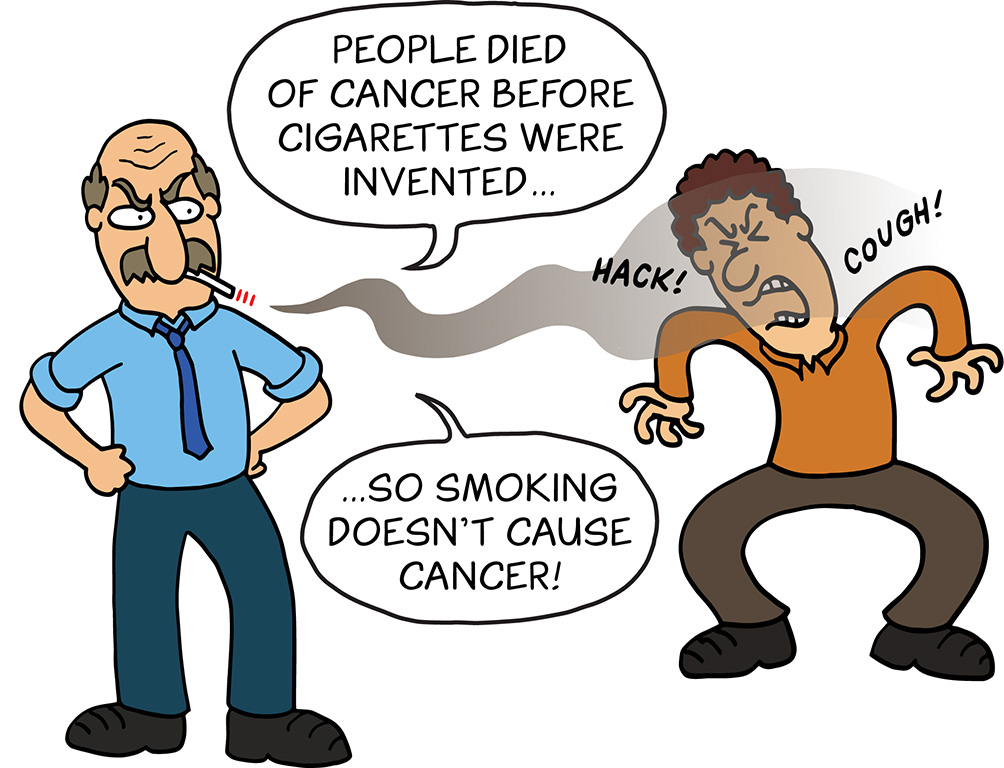
\includegraphics[scale=0.3]{../graphics/smoking-non-sequitur}
\end{figure}


\begin{figure}
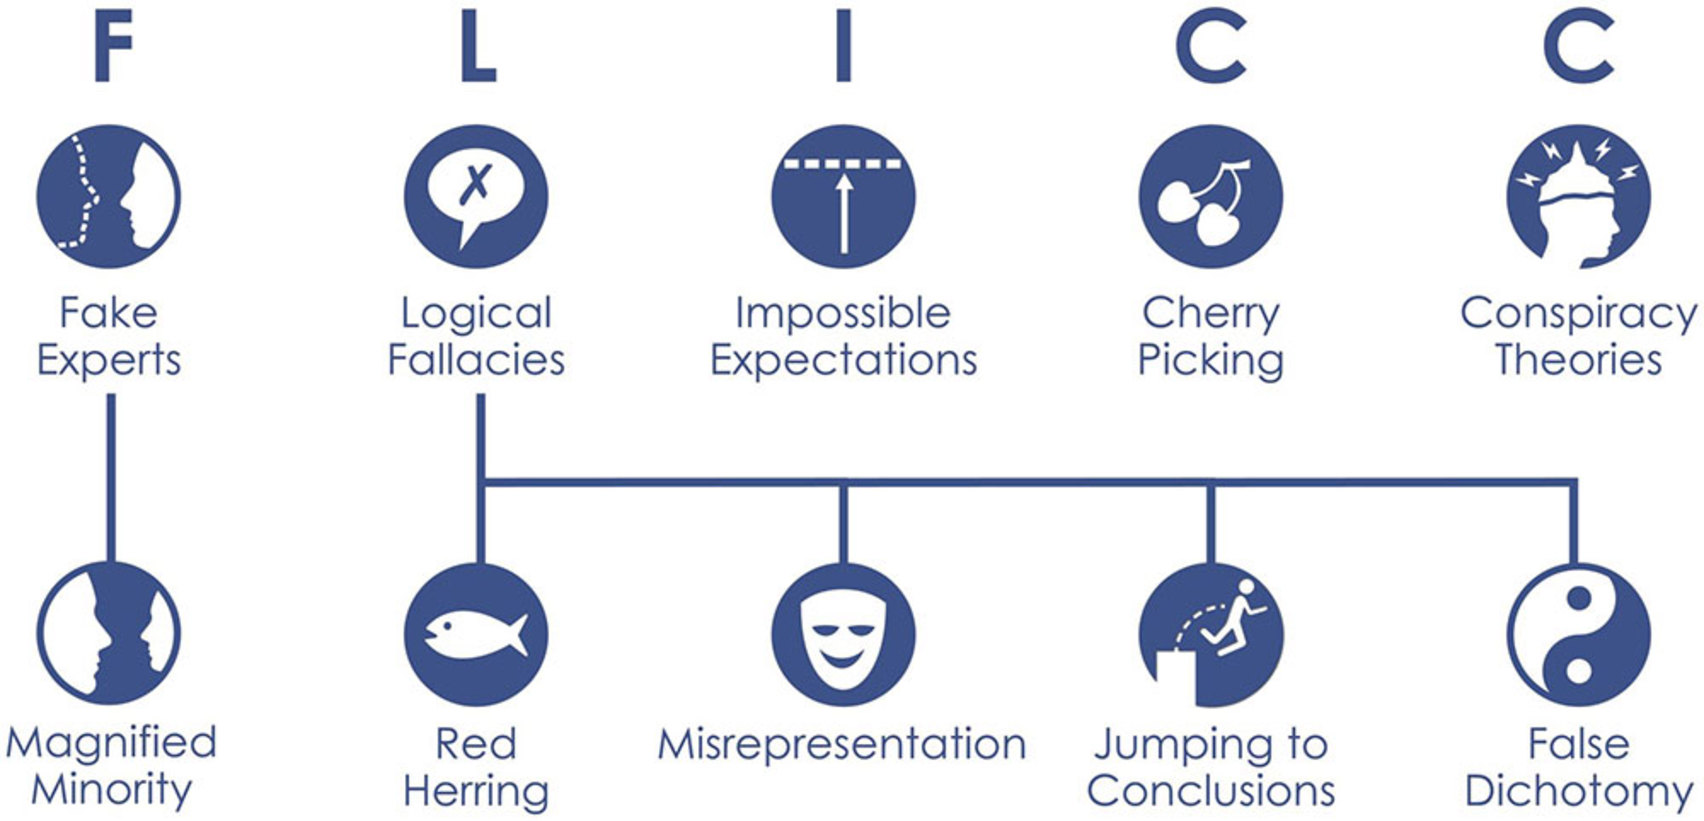
\includegraphics[scale=0.2]{../graphics/skeptical-science-five-traits-science-denial-graphic_creative-commons}
\caption{Source: \url{https://www.desmogblog.com/2017/02/12/what-do-gorilla-suits-and-blowfish-fallacies-have-do-climate-change}.}
\end{figure}

\end{document}
